% ——————————————————————————————————————————————————————————————————
% Оригинальная статья: https://www.nngroup.com/articles/design-thinking/.
% Перевела @rinashm. Приветствуются пуллреквесты для чистки
% синтаксиса и~исправления неточностей перевода. 
% ——————————————————————————————————————————————————————————————————

\documentclass[12pt]{article}

\usepackage{import}
\import{preamble/}{preamble}
\graphicspath{{img/}}

\AtBeginDocument{%
	% Минимальное число букв до переноса
	\lefthyphenmin=3
	% Минимальное число букв после переноса
	\righthyphenmin=3
}

\begin{document}

\title{Основы дизайн"=мышления}
\subtitle{Основы дизайн"=мышления}

\articleauthor{%
	design-thinking-author.jpg%
}{%
	\href{%
		https://www.nngroup.com/articles/author/sarah-gibbons/%
	}{Сара Гиббонс}%
}{%
	31 июля 2016\,г.
	\(\cdot\)
	Пересмотрено 15~июля~2026~г.%
}

\begin{leftbar}
	\large
	\textbf{Кратко:} дизайн"=мышление~"--- это процесс, ориентированный на пользователя, который помогает командам понимать потребности, генерировать идеи, тестировать решения и~способствовать инновациям.
\end{leftbar}

\vspace{0.8em}
{\noindent{\large\fontseries{b}\selectfont Содержание\par}}
\vspace{-0.8em}
\begin{leftbar}
	\vspace{-12pt}
	\tableofcontents
\end{leftbar}

\section{Определение дизайн"=мышления}
Дизайн"=мышление~"--- это \textbf{методология}%
\footnote{%
	В~оригинале автор использует термин \tdef{ideology}~"---
	«идеология», но в~русском языке это слово имеет явно
	выраженный социологический оттенок.%
}%
, подкрепляемая соответствующим процессом. Для полного понимания нужно разобраться в~обоих. 

\begin{leftbar} 
	\textbf{Дизайн"=мышление} утверждает, что прикладной, ориентированный на пользователя подход к~решению проблем, ведёт к~инновациям, а~инновации помогают выделиться на рынке и~получить конкурентное преимущество. Этот прикладной, ориентированный на пользователя подход, определяется \textbf{дизайн"=процессом} и~состоит из шести различных этапов, о~которых будет рассказано ниже.
\end{leftbar}

\section{Процесс}
Фреймворк дизайн"=мышления состоит из трёх шагов:   
\begin{enumerate*}[label=\arabic*)]
	\item understand~"--- понять;
	\item explore~"--- изучить;
	\item materialize~"--- воплотить.
\end{enumerate*}
Внутри этих крупных разделов выделяют~\hyperref[pic:poster]{шесть этапов:}
\begin{enumerate*}[label=\arabic*)]
	\item empathize~"--- эмпатия;
	\item define~"--- фокусировка (определение проблемы);
	\item ideate~"--- генерация идей;
	\item prototype~"--- прототипирование;
	\item test~"--- тестирование;
	\item implement~"--- внедрение.
\end{enumerate*}

\begin{figure}[H]
	\centering
	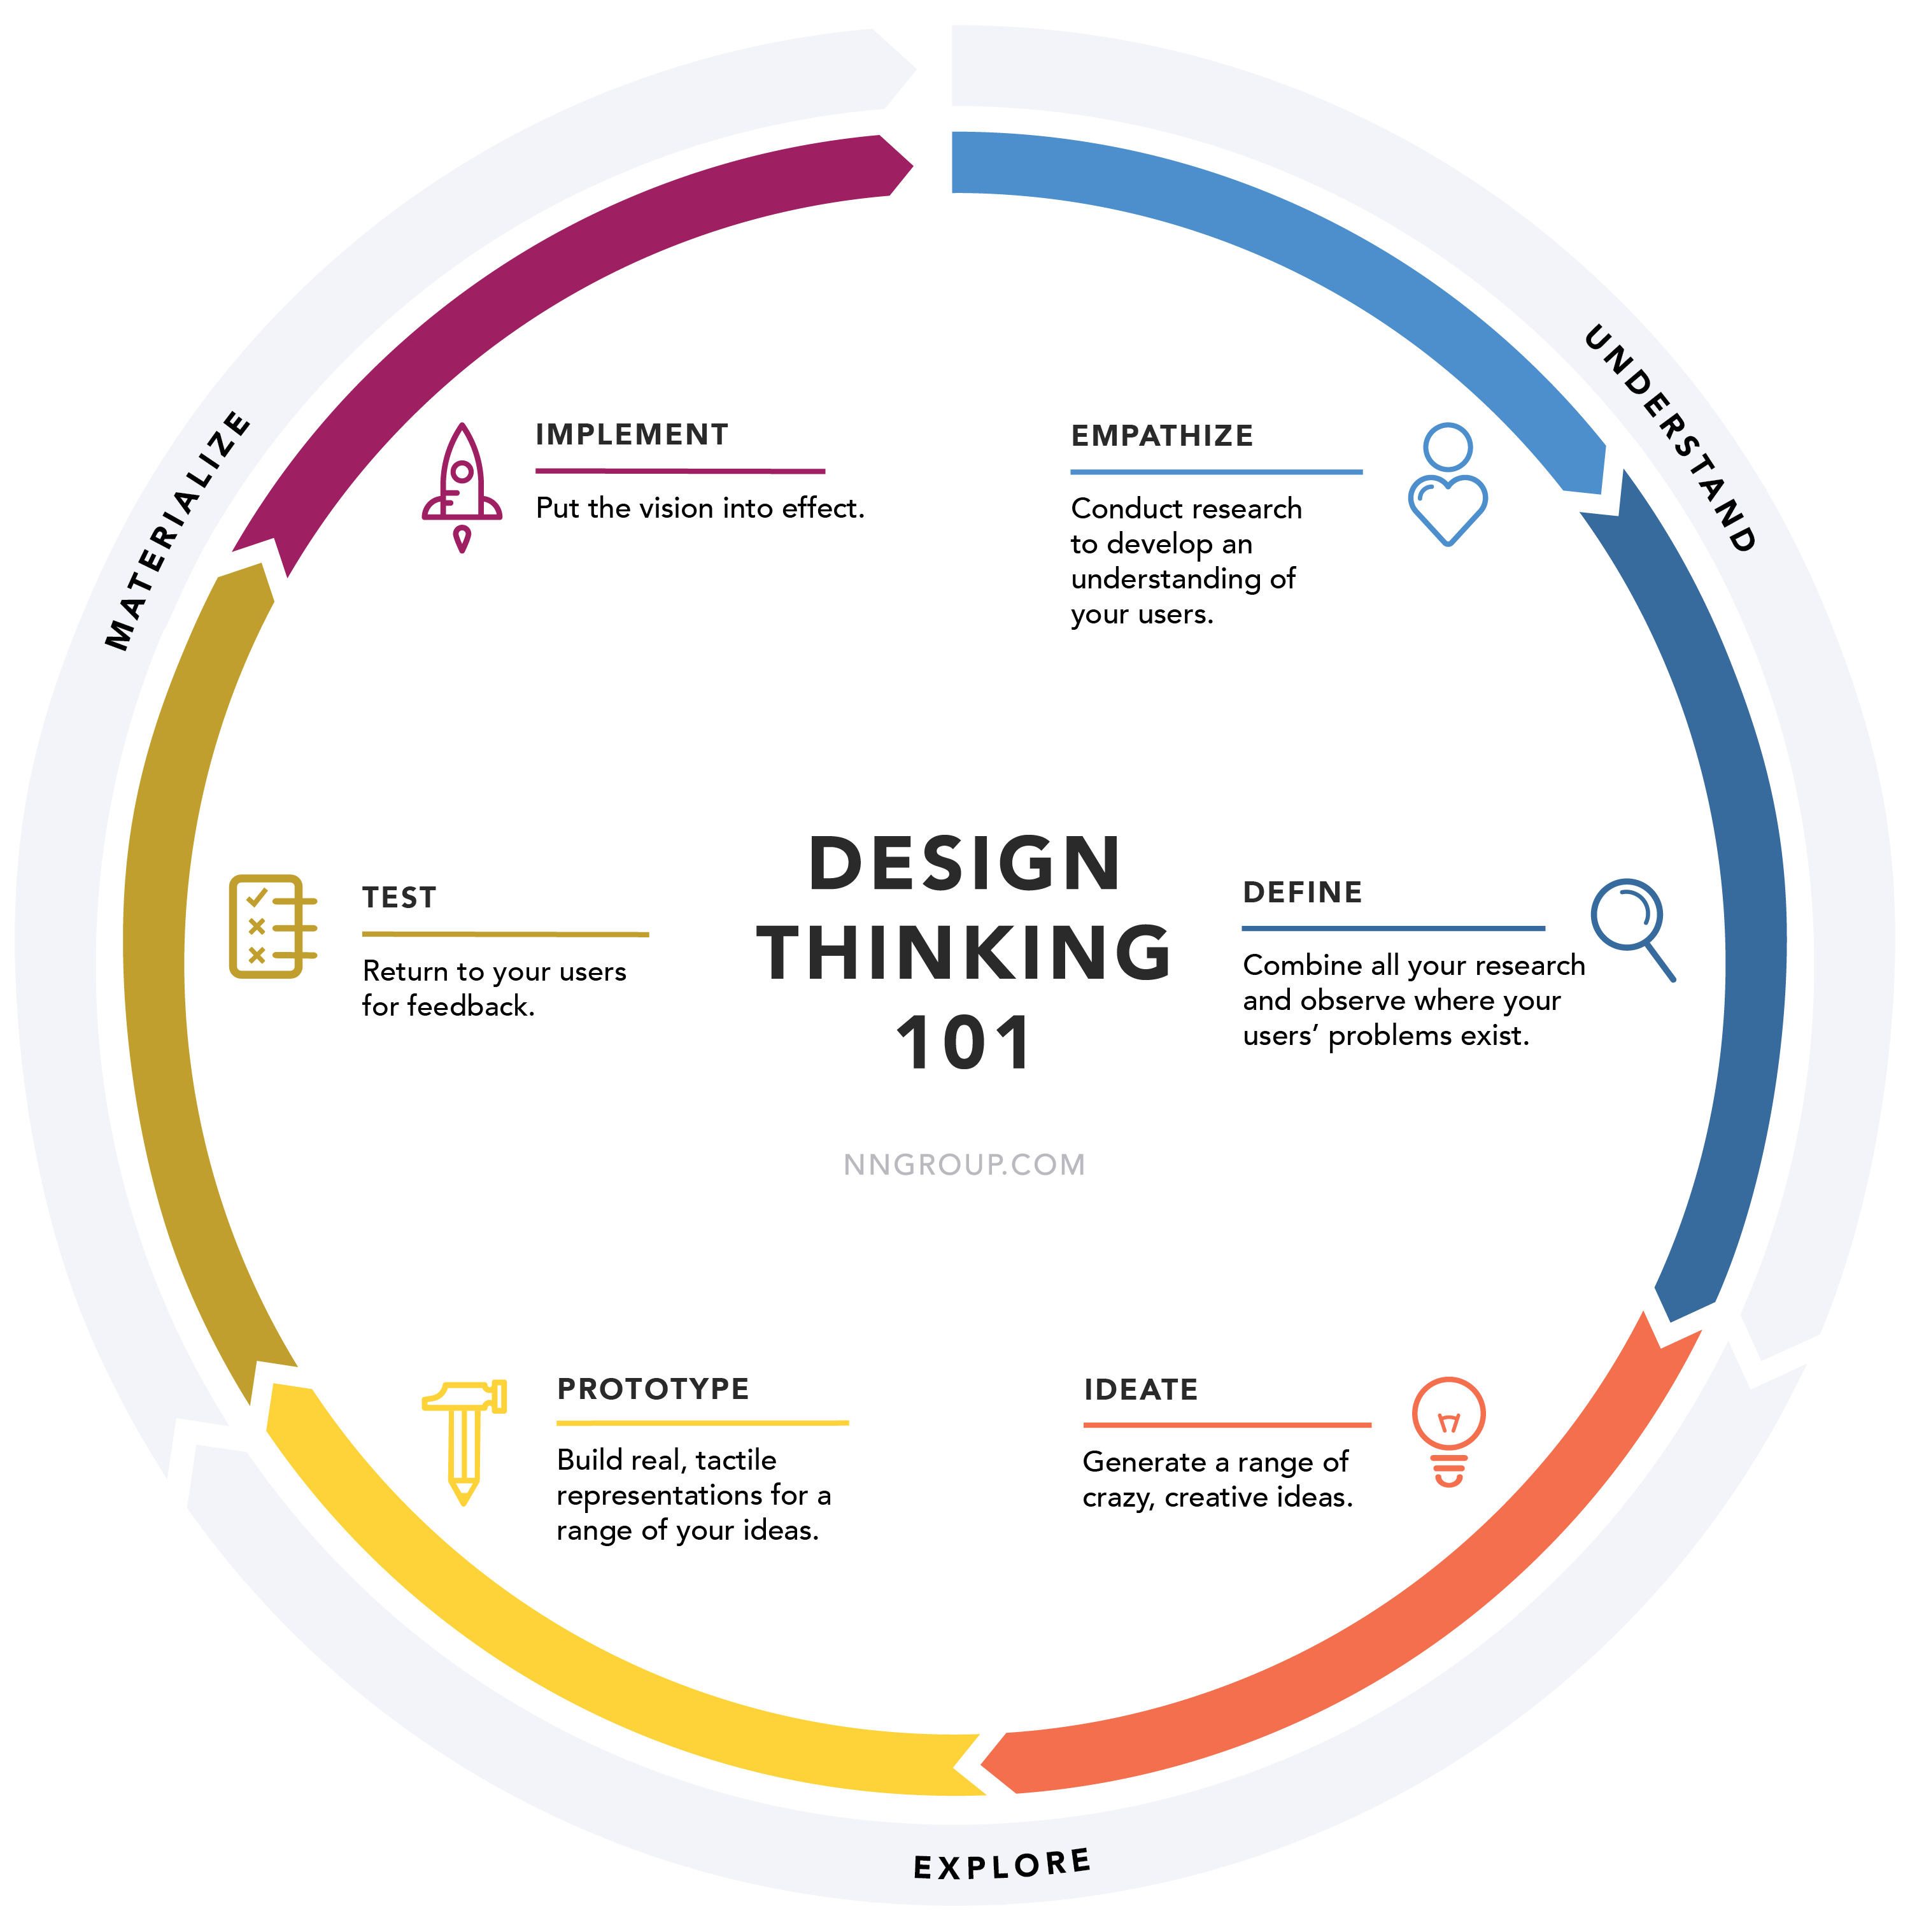
\includegraphics[width=\textwidth]{design-thinking-1.png}
\end{figure}

\subsection*{Эмпатия}

Проведите исследования, \textbf{чтобы разобраться в~том, что ваши пользователи \href{https://www.nngroup.com/articles/empathy-mapping/}{делают, говорят, думают и~чувствуют.}}

Представьте, что ваша цель~"--- улучшить онбординг%
\footnote{%
	\tdef{Онбординг} (в~мобильном приложении)~"--- серия
	приветственных обучающих экранов, которые открываются при
	первом запуске приложения.%
}
для новых пользователей. На этом этапе вы разговариваете с~широким кругом реальных людей. Самостоятельно наблюдайте, что они делают, как думают и~чего хотят; задавайтесь вопросами: «что мотивирует», «что отталкивает», «где люди испытывают раздражение». Ваша задача~"--- собрать достаточно наблюдений, чтобы по"=настоящему сопереживать пользователям и~понимать их точку зрения.

\subsection*{Фокусировка}
Объедините исследования \textbf{и~наблюдайте, где у~пользователей возникают проблемы.} Определяя \href{https://www.nngroup.com/articles/user-need-statements/}{их потребности}, ищите, что можно улучшить.

Вернемся к~примеру с~онбордингом. На этапе фокусировки
используйте всё, что узнали на этапе эмпатии, чтобы найти
инсайты%
\footnote{%
	\tdef{Инсайты} (англ.~\tdef{insights})~"--- внезапная, неочевидная
	информация о~задаче.%
}%
.
Соберите наблюдения воедино и~поищите сходства в~опыте разных пользователей. Есть ли у~них общая болевая точка? Найдите неудовлетворенные потребности ваших пользователей. 

\subsection*{Генерация идей}
\textbf{Проведите мозговой штурм: придумывайте безумные, креативные идеи,} которые закрывают неудовлетворенные потребности пользователей из предыдущего этапа. Дайте себе и~команде полную свободу: не критикуйте идеи, чем их больше~"--- тем лучше.

На этом этапе соберите команду, чтобы вместе придумать как можно больше идей. Пусть участники делятся ими, смешивают и~дополняют друг друга.

\subsection*{Прототипирование}
Возьмите часть идей и~сделайте их осязаемыми. Цель этого этапа~"--- \textbf{понять, что сработает,} а~что~"--- нет. На этом этапе вы начинаете сопоставлять значимость и~реализуемость своих идей, опираясь на комментарии к~прототипам. 

Сделайте вашу идею осязаемой. Если это новый лендинг, нарисуйте его вайрфрейм и~соберите обратную связь от команды. Внесите правки, а~затем еще раз соберите быстрый прототип, не беспокоясь о~качестве программного кода. Затем покажите его другой группе людей.  

\subsection*{Тестирование}
Вернитесь к~пользователям за обратной связью. Спросите себя: «Это решение соответствует потребностям пользователей?» и~«Улучшает ли оно то, как они себя чувствуют, думают и~выполняют действия?».

\textbf{Покажите прототип реальным клиентам} и~убедитесь, что он решает поставленные задачи. Улучшился ли опыт пользователей во время онбординга? Увеличивает ли новый лендинг время или деньги, которые человек тратит на сайте? Продолжайте тестировать свое решение по ходу реализации.

\subsection*{%
	Внедрение%
	\footnote{%
		В~оригинальной статье этот этап не~был вынесен в~подраздел,
		но должен тут быть с~точки зрения смысла
	}%
}

Претворите вашу идею в~жизнь. Убедитесь, что решение реализовано и~затрагивает жизнь конечного пользователя.

Это самая важная часть дизайн"=мышления, но о~ней часто забывают. Как настаивает Дон Норман: «нам нужно больше \emph{делать} дизайн»%
\footnote{%
	``We need more design doing''.%
}%
. Дизайн"=мышление не освобождает от того, чтобы реально делать дизайн. Это не волшебство. 
\par

\begin{leftbar}
	«Не бывает „творческих натур“. Креативность~"--- это глагол,
	и~очень времязатратный. Это означает взять идею в~своей
	голове и~сделать её реальной. И~всегда это долгий и~сложный
	процесс. Если делать всё правильно, это ощущается как
	работа»~"--- Милтон Глейзер%
	\footnoteen{%
			``There’s~no such thing as a~creative type. As if creativity
			is a~verb, a~very time-consuming verb. It’s~about taking
			an idea in your head, and transforming that idea into
			something real. And that’s~always going to be a~long and
			difficult process. If you’re doing it right, it’s~going to
			feel like work''.%
	}
\end{leftbar}

Как бы важно ни было дизайн"=мышление для организации, оно ведет к~настоящим прорывам только если идея реализована. Успех дизайн"=мышления определяется тем, может ли оно повлиять на жизнь конечного пользователя. Шестой шаг~"--- внедрение~"--- имеет решающее значение.  

\section{В~чём преимущество}

Зачем по"=новому подходить к~разработке продукта? Есть множество причин погрузиться в~дизайн"=мышление, достойных отдельной статьи, но вкратце: дизайн"=мышление даёт \textbf{все} эти преимущества одновременно.

Дизайн"=мышление:
\begin{itemize}

	\item\textbf{это ориентированный на пользователя процесс}, который начинается с~данных о~пользователе, создаёт дизайн"=артефакты, которые закрывают настоящие, а~не воображаемые потребности людей, и~тестирует эти артефакты с~реальными пользователями;

	\item\textbf{опирается на опыт и~знания команды,} формирует общий язык и~вовлечённость команды;

	\item\textbf{мотивирует придумывать новое,} исследуя несколько путей решения одной и~той же задачи.
\end{itemize}

Якоб Нильсен говорит:
\href{%
	https://www.nngroup.com/articles/the-myth-of-the-genius-designer/%
}{%
	«Восхитительный интерфейс, решающий не ту
	задачу, провалится»%
}%
\footnote{%
	``A~wonderful interface solving the wrong problem will fail''.%
}.
Дизайн"=мышление высвобождает творческую энергию и~направляет её на нужную проблему.

\section{Гибкость: подстроится под ваши потребности}

Поначалу описанный выше процесс будет казаться замысловатым. Не~думайте о~нём как о~пошаговой инструкции для успеха. Вместо этого используйте его как опору там и~когда это нужно. Будьте шеф"=поваром, а~не поваром фастфуда: берите рецепт как фреймворк и~меняйте, как вам нужно.

Каждый этап задуман не как строго линейный, а~как итеративный (выполняется в~несколько подходов) и~цикличный. Команды часто возвращаются к~двум первым этапам понимания потребностей пользователей~"--- эмпатии и~фокусировке~"--- после того как собрали и~протестировали начальный прототип. Это происходит, потому что вы получаете точную картину своего дизайна только после того, как вайрфреймы собраны в~прототип и~идея воплощена в~жизнь. Впервые вы можете точно оценить, работает ли ваше решение. Вернувшись к~исследованиям, вы поймёте, чего ещё не знаете о~пользователях, чтобы принять решения или расставить приоритеты разработки. Ещё вы случайно можете обнаружить новые кейсы из~прототипа, которые не~изучались ранее.

При необходимости этапы можно повторить. Часто, пока команда не получит нужный результат, участники по нескольку раз возвращаются к~практическим задачам в~рамках одного и~того же этапа. На~этапе фокусировки может оказаться, что у~членов команды разный опыт, экспертиза и~подходы к~выявлению проблем. Если задержаться тут, можно прийти к~общему пониманию цели, особенно когда трудно заручиться поддержкой всей команды. Каждый этап должен выдавать достаточно крепкий результат, чтобы служить ориентиром для~следующих этапов и~не давать команде сбиваться с~курса.

\section{Масштабируемость: помогает мыслить шире}

Компактность и~доступность дизайн"=мышления делают его масштабируемым. Организации, до этого не~способные изменить свой стиль мышления, получили инструкцию, понятную вне зависимости от~уровня экспертности. Она сглаживает различия в~мастерстве дизайнеров, повышая шансы на~успех. Дизайн"=мышление можно применить не только к~традиционным «дизайнерским» сферам вроде продуктового дизайна, но~и~к~широкому кругу социальных, экологических и~экономических проблем. Дизайн"=мышление достаточно просто, чтобы использоваться в~проблемах различного масштаба, даже для сложных, неопределяемых и~иначе непосильных задач. Его можно применять для небольших улучшений, например, строки поиска, и~в~то же время~"--- для прорывных, трансформирующих решений, например реорганизация карьерной лестницы учителей таким образом, чтобы сохранять талантливых педагогов.

\section{История дизайн"=мышления}

Люди ошибочно полагают, что дизайн-мышление~"--- новое явление, однако дизайн присутствует в~нашей жизни веками. Памятники, мосты, автомобили, метро~"--- результаты работы дизайнеров. На протяжении истории хорошие дизайнеры вводили в~свою практику человекоцентричный творческий процесс, создавая важные и~эффективные решения.

В~ранние 1900-е~супруги и~дизайнеры Чарльз и~Рэй Имз занимались тем, что можно назвать «изучением в~процессе работы». Они изучали потребности и~возможности людей, пока не создали знаменитые стулья Eames, которые можно найти в~магазинах и~семьдесят лет спустя. Модельер Джин Мьюир, работавшая в~1960-х~годах, была известна «здравым смыслом» в~дизайне одежды. Её интересовало не только то, как вещи выглядели для других, но и~то, удобно ли в~них ходить. Эти дизайнеры были новаторами своего времени. Их подходы называют ранними примерами дизайн-мышления: каждый разбирался в~сценариях и~думал о~неудовлетворенных потребностях пользователей. Милтон Глейзер, автор знаменитого логотипа I~$\heartsuit$~NY, хорошо описал эту мысль: «Мы всё время на что-то смотрим, но редко по-настоящему видим,
$\left<\dots\right>$
именно направление внимания позволяет по-настоящему постичь что-то, полностью это осознать».

Несмотря на эти и~другие ранние примеры человекоориентированного дизайна, в~бизнесе его долгое время использовали лишь для улучшения внешнего вида продукта. Из-за такого поверхностного подхода решения не учитывали реальные потребности людей. Постепенно часть компаний начали привлекать дизайнеров в~начале разработки продукта, а~не в~самом конце, где их вклад был ограничен. Компании, использующие ориентированный на пользователя подход, зарабатывали больше на продуктах, которые удовлетворяли потребности клиентов.

Чтобы применять такой подход в~крупных организациях нужны были стандарты. Так и~появилось дизайн-мышление~"--- подход, который помогает использовать методы креативного дизайн-процесса в~для решения различных бизнес-задач.

Сам термин «дизайн-мышление» был введён в~1990-х~годах Дэвидом Келли и~Тимом Брауном из IDEO вместе с~Роджером Мартином. Идеи и~методы, которые развивались годами, постепенно объединились в~более целостный подход.


\section*{Заключение}

Мы живём в~эпоху важности пользовательского опыта, будь то сервис или продукт. У~нас высокие ожидания от этого опыта.  Продукты усложняются, а~данные и~технологии продолжают развиваться. С~каждым витком эволюции появляются новые неудовлетворённые потребности. Дизайн"=мышление~"--- это всего лишь подход к~решению проблем, но он увеличивает ваши шансы на успех и~создание чего-то прорывного.

\begin{figure}[H]
	\centering
	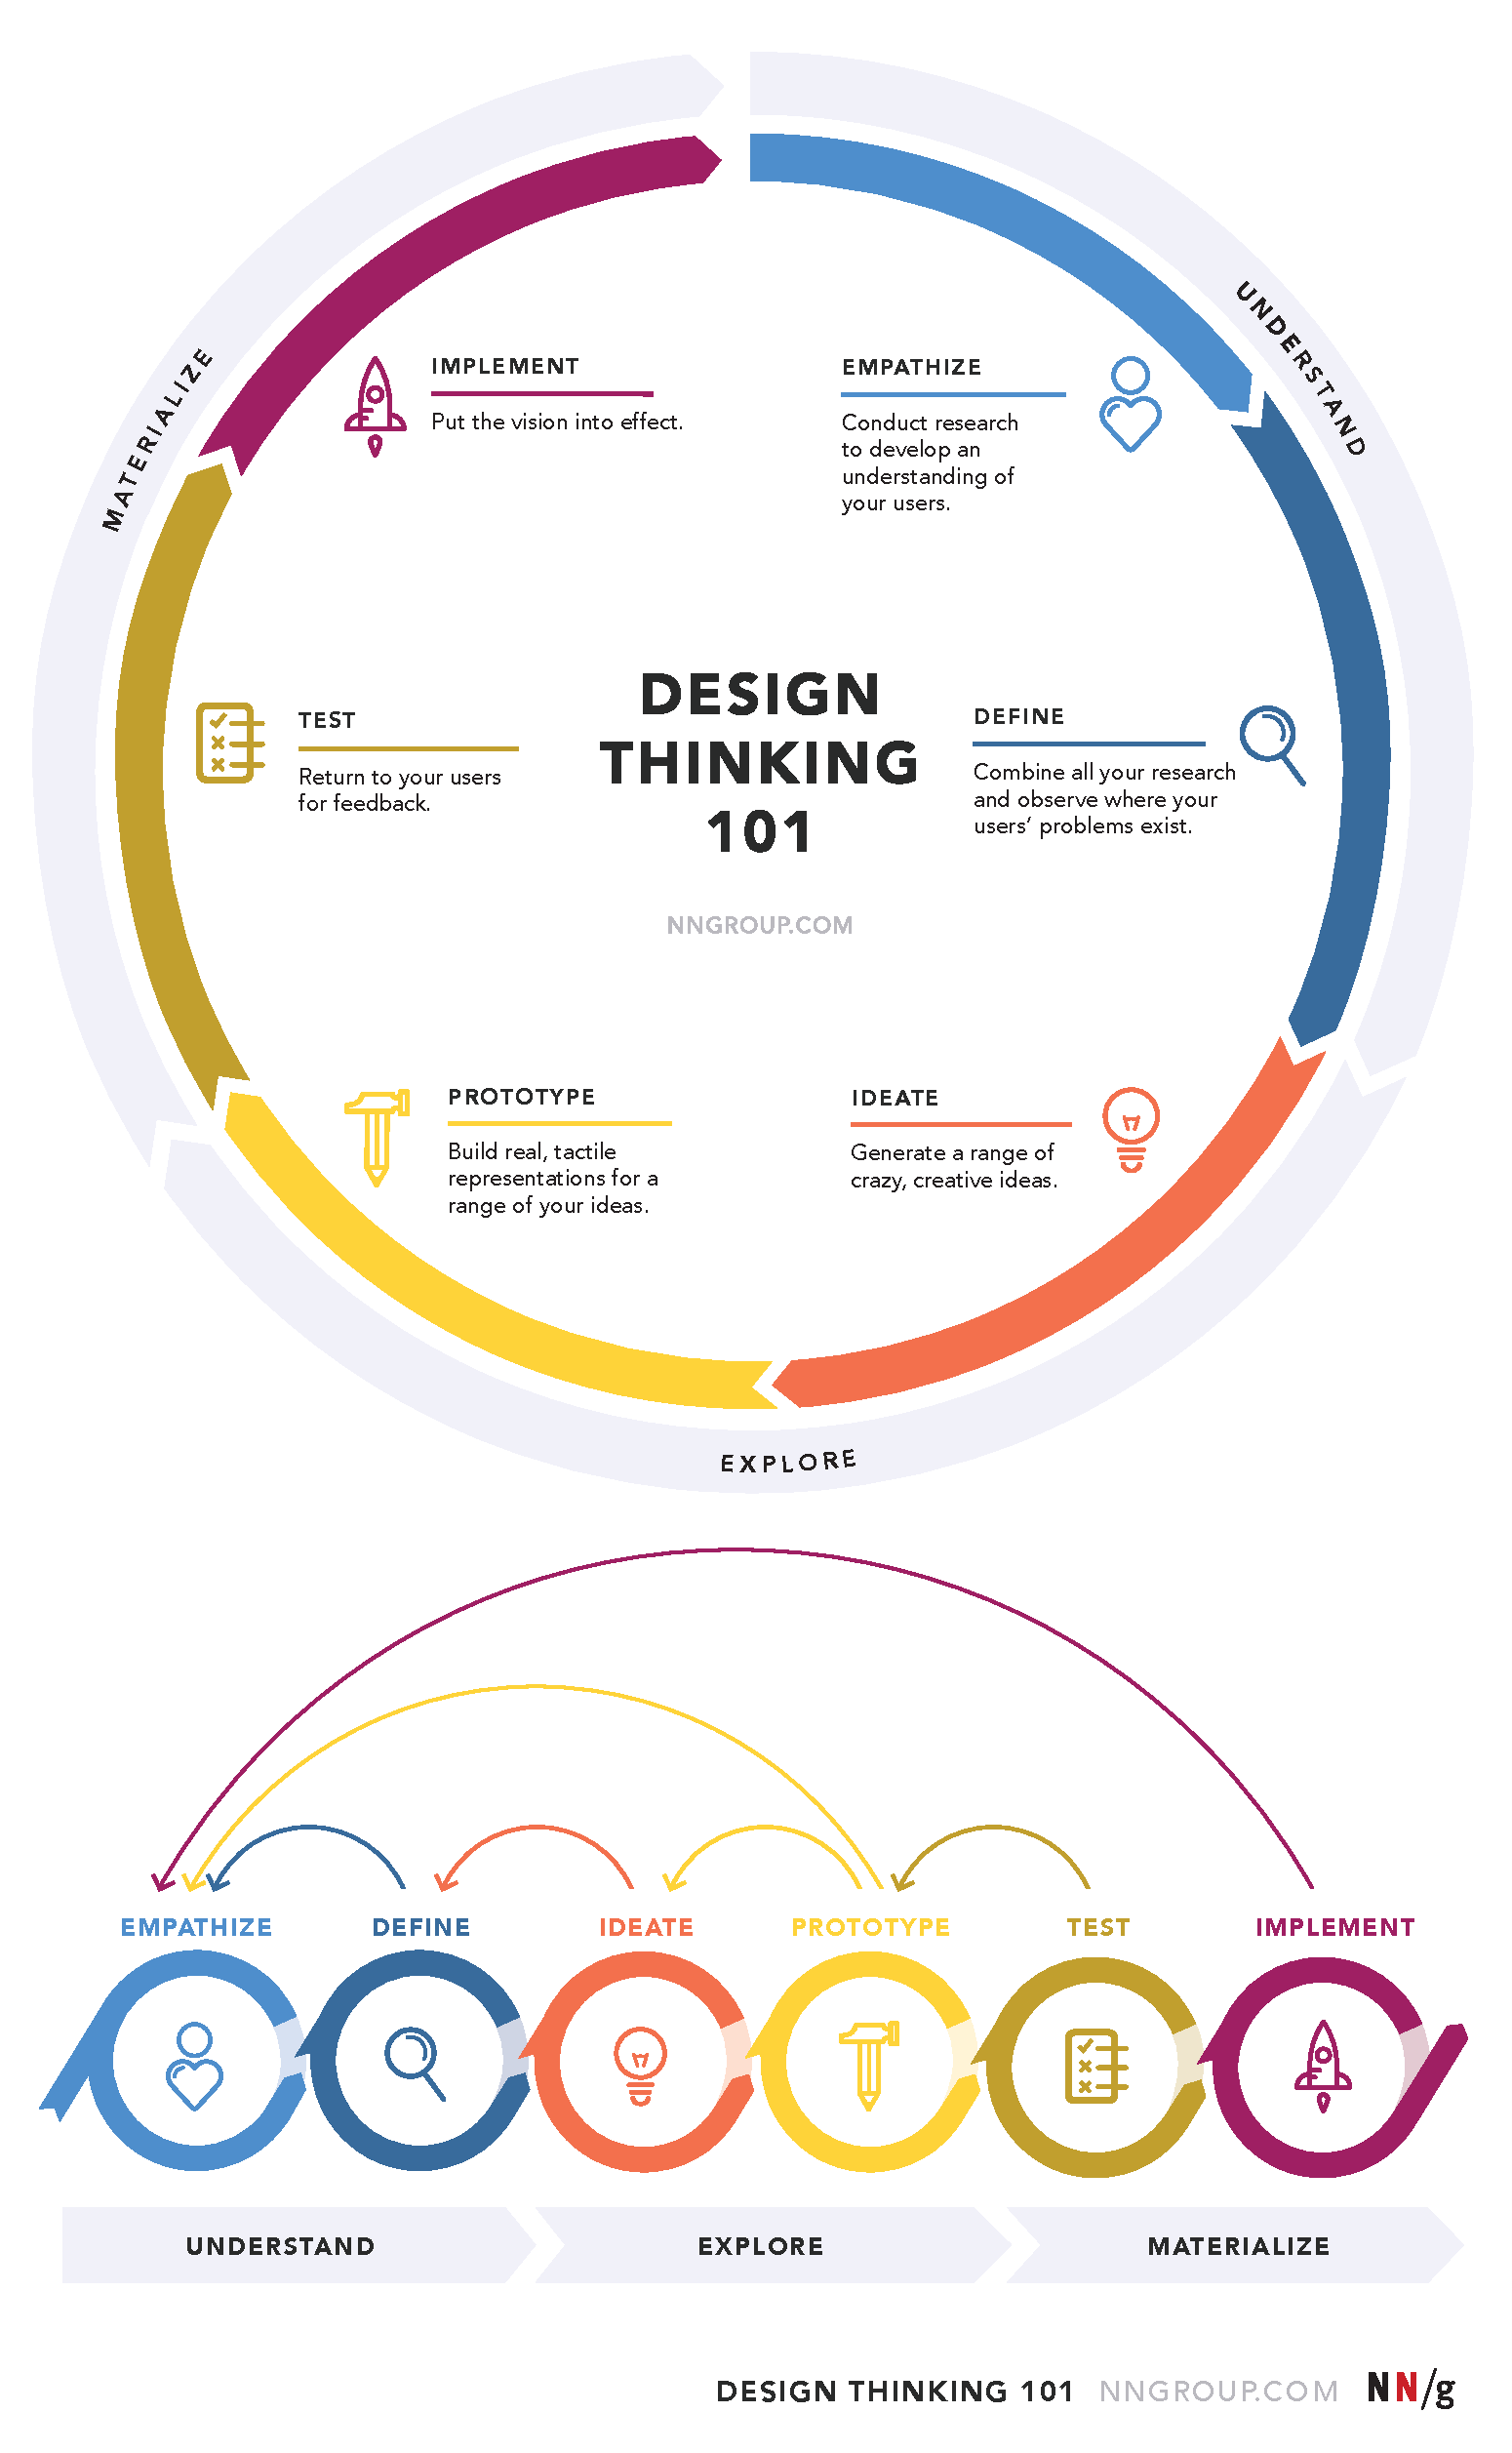
\includegraphics[width=\textwidth, height=0.85\textheight, keepaspectratio]{Design-thinking-101-NNG.pdf}
	\par
	\vspace{2em}
	\mbox{%
		\fontfamily{far}%
		\selectfont
		\href{%
			https://media.nngroup.com/media/articles/attachments/Design-thinking-101-NNG.pdf
		}{Design Thinking (PDF)}%
	}
	\label{pic:poster}
\end{figure}

\end{document}

% vim:ts=2:sw=2
